\Chapter{Projektablauf}
Zu Beginn des Projekts wurde eine Unterteilung der Anforderungen in ein
Basisangebot sowie ein daran ankn\"upfendes Erweiterungsangebot vollzogen.
W\"ahrend innerhalb des ersten Semesters vor allem der
Eingew\"ohnung in die Entwicklungsumgebung und Realisierung der Basisziele diente,
sah die Planung f\"ur das zweite Semester eine Erweiterung des dann bereits
lauff\"ahigen Prozessors um zus\"atzliche Module vor. 

\Section{Aufgabe}
Die Hauptaufgabe bestand darin, eine Implementierung eines funktionsf\"ahigen
Prozessor auf Basis der
\href{https://riscv.org/specifications/}{RISC-V Instruction Set Architecture}
anzufertigen, welche auf dem zur Verf\"ugung gestellten Entwicklungsboard
(\textit{Spartan-3A FPGA Starter Kit}) lauff\"ahig sein sollte.

\begin{figure}[H]
\centering
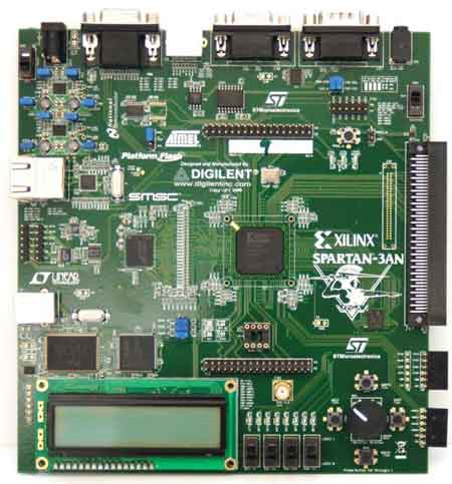
\includegraphics[width=0.3\textwidth]{Board.png}
\caption{Das verwendete Entwicklungsboard von oben, das FPGA liegt zentral}
\label{fig:board}
\end{figure}

\Section{Basisziele}
Als Mindestanforderung sollte dabei die Kompatibilit\"at zur
\textit{RV32I Base Integer Instruction Set} gew\"ahrleistet werden. Ausgenommen
davon waren die speziell f\"ur Aspekte des Multithreadings auf
Mehrkernprozessoren enthaltenen Befehle \Instr{FENCE}, \Instr{FENCE.I},
\Instr{SCALL} und \Instr{SBREAK}, da die geforderte Implementierung lediglich
einen Rechenkern besitzen sollte.

Um die Funktionsf\"ahigkeit des Prozessors auch nach au\ss{}en hin sichtbar zu
machen und damit einhergehend keine Black-Box Komponente zu entwickeln, sollte
eine M\"oglichkeit zur Benutzerinteraktion \"uber geeignete, auf dem
Entwicklungsboard vorhandene Bausteine wie etwa Schalter bestehen. Insbesondere
zu Zwecken des Debuggings wurde auch eine grafische Ausgabe der internen
Register \"uber die VGA-Schnittstelle zu einem angeschlossenen Monitor
inkludiert.
\footnote{Siehe dazu auch Pflichtenheft vom 02.06.16 bzw. 12.11.16}

\Section{Erweiterungsziele}
Die Modularit\"at der RISC-V ISA legt einige sinnvolle Erweiterungen nahe,
darunter auch die
\textit{RV32M Standard Extension for Integer Multiplication and Division},
welche Multiplikations- und Divisionsbefehle beinhaltet. Zudem sollte die
rudiment\"are Ausgabe der internen Register um einen Textmodus erweitert
werden, sodass mittels Memory-Mapping nun auch ASCII-Zeichen auf dem Monitor
ausgegeben werden k\"onnen. Weiterhin wurde, um eine bessere Interaktion mit
dem Programmierer zu erm\"oglichen, auch die Umsetzung einer seriellen
Schnittstelle in den geplanten Erweiterungsrahmen miteinbezogen. Zuletzt
stellt auch das Entwerfen eines demonstrativen Programms, genauer eines
einfachen Spiels, einen ma\ss{}geblichen Bestandteil des Erweiterungsangebots
dar, mit dem Ziel die endg\"ultige Implementierung ad\"aquat pr\"asentieren zu k\"onnen.
\footnote{Siehe Fu\ss{}note 1}

\Section{Projektablauf}
\Subsection{Chronologischer Verlauf}
Wie eingangs erw\"ahnt umfasste die Dauer des Praktikums zwei Semester, in
denen im Allgemeinen drei verschiedene Implementierungsversionen angefertigt
wurden.

\begin{table}[H]
\begin{tabular}{|p{45pt}|p{80pt}|p{220pt}|p{115pt}|}
\hline
Version                                  & Zeitraum                                 & Ziele                                                                      & davon nicht erreicht                     \\
\hline
\begin{description}[noitemsep,topsep=0pt]
\item 1
\end{description}                        & \begin{description}[noitemsep,topsep=0pt]
                                           \item April 2016 -
                                           \item Juni 2016
                                           \end{description}                        & \begin{itemize}[noitemsep,topsep=0pt]
                                                                                      \item Pr\"ufung der Strukturierung des Prozessors in ALU, Leitwerk und MMU
                                                                                      \item Pr\"ufung der Arbeitsaufteilung
                                                                                      \item Verst\"andnis der Tools
                                                                                      \item Ausf\"uhrung einiger einfacher Befehle
                                                                                      \end{itemize}                                                              &                                          \\
\hline
\begin{description}[noitemsep,topsep=0pt]
\item 2
\end{description}                        & \begin{description}[noitemsep,topsep=0pt]
                                           \item Juni 2016 -
                                           \item September 2016
                                           \end{description}                        & \begin{itemize}[noitemsep,topsep=0pt,itemindent=0pt]
                                                                                      \item Implementierung der RV32I-Spezifikation
                                                                                      \item Lese- und Schreibzugriff auf den DDR2-RAM
                                                                                      \item Debugging-Ausgabe
                                                                                      \end{itemize}                                                              & \begin{description}[noitemsep,topsep=0pt]
                                                                                                                                                                   \item Lese- und Schreibzugriff
                                                                                                                                                                   \item auf den DDR2-RAM
                                                                                                                                                                   \end{description}                        \\
\hline
\begin{description}[noitemsep,topsep=0pt]
\item 3
\end{description}                        & \begin{description}[noitemsep,topsep=0pt]
                                           \item September 2016 -
                                           \item Januar 2017
                                           \end{description}                        & \begin{itemize}[noitemsep,topsep=0pt]
                                                                                      \item Implementierung der RV32M-Spezifikation
                                                                                      \item Lese- und Schreibzugriff auf den DDR2-RAM
                                                                                      \item ASCII-Ausgabe
                                                                                      \item Zugriff auf Buttons, LEDS, \dots{} des Boards durch Memory-Mapped-I/O
                                                                                      \item serielle Schnittstelle (UART)
                                                                                      \end{itemize}                                                              & \begin{description}[noitemsep,topsep=0pt]
                                                                                                                                                                   \item serielle Schnittstelle
                                                                                                                                                                   \item (nur teilweise)
                                                                                                                                                                   \end{description}                        \\
\hline
\end{tabular}
\caption{\"Ubersicht \"uber den Projektablauf}
\end{table}

\Subsection{Arbeitsteilung und Entscheidungsprozesse}
Gem\"a\ss{} den vier Prinzipien der Von-Neumann-Architektur wurde die
Implementierung grob in die Hauptkomponenten Leit-, Rechen-,
Ein-/Ausgabewerk und Speicher gegliedert, was sich konkret in den drei
Subkomponenten CU\ref{ch:cu}, ALU\ref{ch:alu} und MMU\ref{ch:mmu}
widerspiegelt. F\"ur jeden dieser Bausteine war durchg\"angig eine
unabh\"angige Kleingruppe verantwortlich, wobei es trotzdem f\"ur sinnvoll
erachtet wurde, w\"ochentliche Treffen zu Zwecken der Planung und Integration
der Komponenten sowie zum Testen, zu veranschlagen. Entscheidungen von
gr\"o\ss{}erer Tragweite, besonders im Hinblick auf generelle
Designentscheidungen wurden meist im Plenum besprochen.

\Section{Verwendete Tools}
Das Projekt wurde in der Hardwarebeschreibungssprache VHDL implementiert, was
sich darin begr\"undet, dass dieser Themenkomplex Teil der zugrundeliegenden
Lehrveranstaltung war und die Gruppenmitglieder daher auf einem
einigerma\ss{}en gleichwertigen Kenntnisstand waren.

Zur Entwicklung wurde haupts\"achlich die Entwicklungsumgebung Xilinx'
\textit{ISE Project Navigator} in Version 14.7 verwendet. Diese erm\"oglichte
einerseits das Editieren des VHDL-Codes und beinhaltete andererseits auch eine
integrierte Toolchain, um den VHDL-Code in ein Programming-File zu
\"ubersetzen. Dieses wurde dann benutzt, um das Board zu programmieren. Der
zus\"atzlich enthaltene \textit{Core Generator} wurde dabei verwendet, um
einzelne Subkomponenten wie beispielsweise eine Divisionseinheit zu generieren.

\begin{figure}[H]
\centering
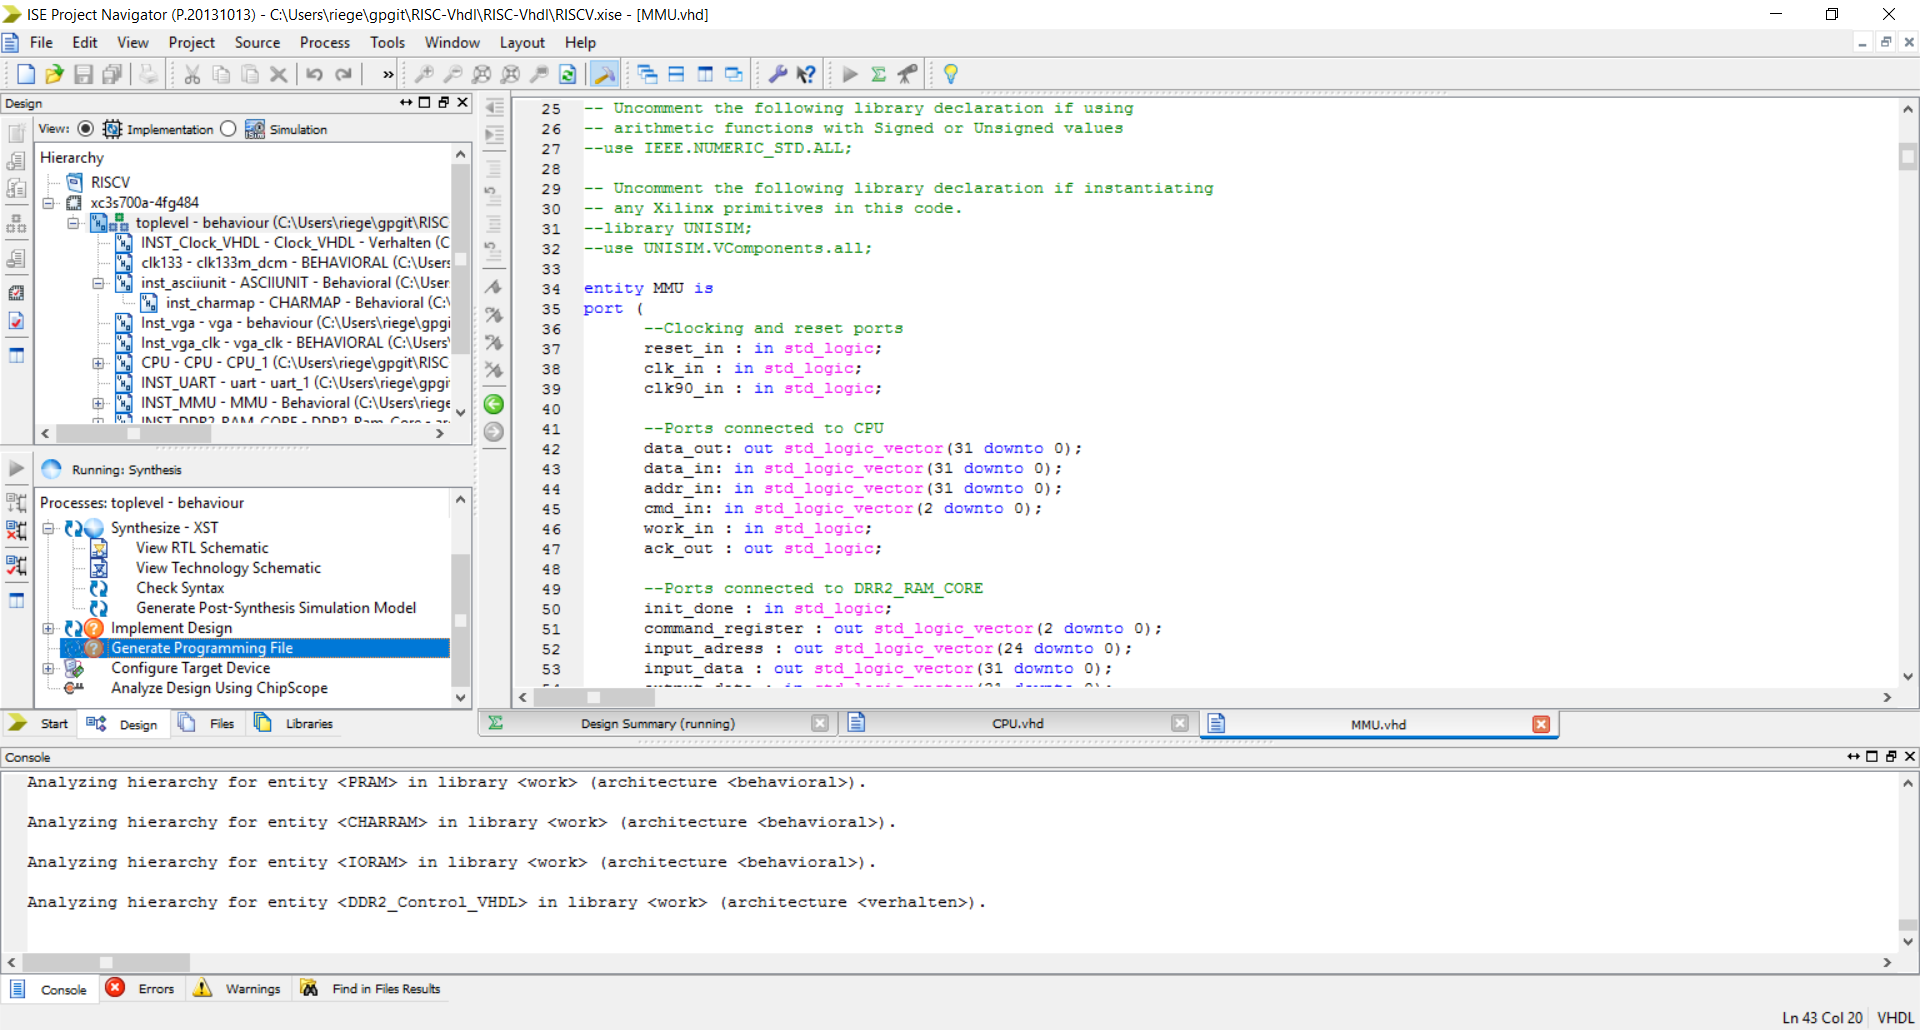
\includegraphics[width=1.0\textwidth]{ISE.png}
\caption{Der Xilinx ISE Project Navigator}
\label{fig:tool}
\end{figure}

Mittels des Tools \textit{impact}, welches ebenfalls vom Anbieter der
Entwicklungsumgebung Xilinx stammt, konnte in Kombination mit einem
\textit{Cable-Server} das Board \"uber USB gem\"a{\ss} den erstellten
Programming-Files beschrieben werden. Zur Versionsverwaltung wurde dabei
auf ein \textit{Git-Repository} gesetzt.

Um die doch recht umfassende Arbeit des Assemblierens eines Programms nicht
h\"andisch erledigen zu m\"ussen, wurde, wie sp\"ater genauer erl\"autert wird,
ein automatischer Assemblierer in der Skriptsprache Python entwickelt. Da die
Generierung eines Programming-Files und das anschlie\ss{}ende Beschreiben des
FPGAs nichtsdestotrotz jedes Mal mehrere Minuten in Anspruch nahm,
wurden entsprechende Simulatoren verwendet. Zur Verifikation des VHDL-Codes
wurde beispielsweise das Tool \textit{GHDL} in Kombination mit \textit{GTKWave}
benutzt. Auch zum Testen der Assemblerprogramme wurde ein Simulator auf
Python-Basis, der die Umgebung des Boards emuliert, entworfen und in den
Arbeitsprozess mit eingebunden.
